\section{A Pragmatic Journey: Why Trained Models Failed}
\label{sec:journey}

Before committing to the VLM pipeline of Sec.~\ref{sec:system}, we tried
four families of trained and physics-based approaches. Each worked in
isolation on curated tutorial clips and broke on real competition footage.
We describe them compactly here because every failure motivates a specific
design choice in the VLM pipeline.

\paragraph{v1 --- 2D pose + hand-crafted physics.}
Our first pipeline ran ViTPose~\cite{xu2022vitpose} for 2D keypoints and
classified tricks from hand-computed torso angles and ankle asymmetry.
Clean side-on tutorial clips worked; the brittleness appeared the moment
the camera moved or the athlete was shot from behind. 2D rotation axes are
projections, and the ambiguity between, e.g., a cork and a back full is
fundamental in the image plane.

\paragraph{v2--v4 --- GVHMR 3D mesh + rotation decomposition.}
We then replaced the 2D front-end with GVHMR~\cite{shen2024gvhmr}, which
returns world-aligned SMPL parameters, and computed per-frame swing/twist
decomposition from the global orientation quaternion. On close-up single-trick
clips the pipeline measured flip and twist counts to within 10\% of the
expected values for back flips, front flips, and gainers. On real
competition footage it collapsed: total rotation was inflated by up to
76\,\% on off-axis tricks such as double corks, body shape classification
misread layouts as tucks, and the system reported ``forward'' direction for
unambiguously backward flips. Deep inspection confirmed the cause:
GVHMR~--- like WHAM, TRAM, and TokenHMR~--- is trained on
AMASS~\cite{mahmood2019amass}, which contains \emph{zero} acrobatic
sequences. Figure~\ref{fig:gvhmr_failure} shows the mesh exploding on the
double-cork clip.  Berry-phase correction, quaternion smoothing, and
snap-to-half post-processing all reduced noise but could not compensate for
fundamentally out-of-distribution inputs.

\paragraph{Lesson.} Building increasingly ornate post-processing on broken
physics is a dead end. The fix is either a new 3D model fine-tuned on
acrobatic data (a whole research project in itself) or moving up the
abstraction hierarchy to a system that does not need frame-level 3D at all.

\begin{figure}[t]
  \centering
  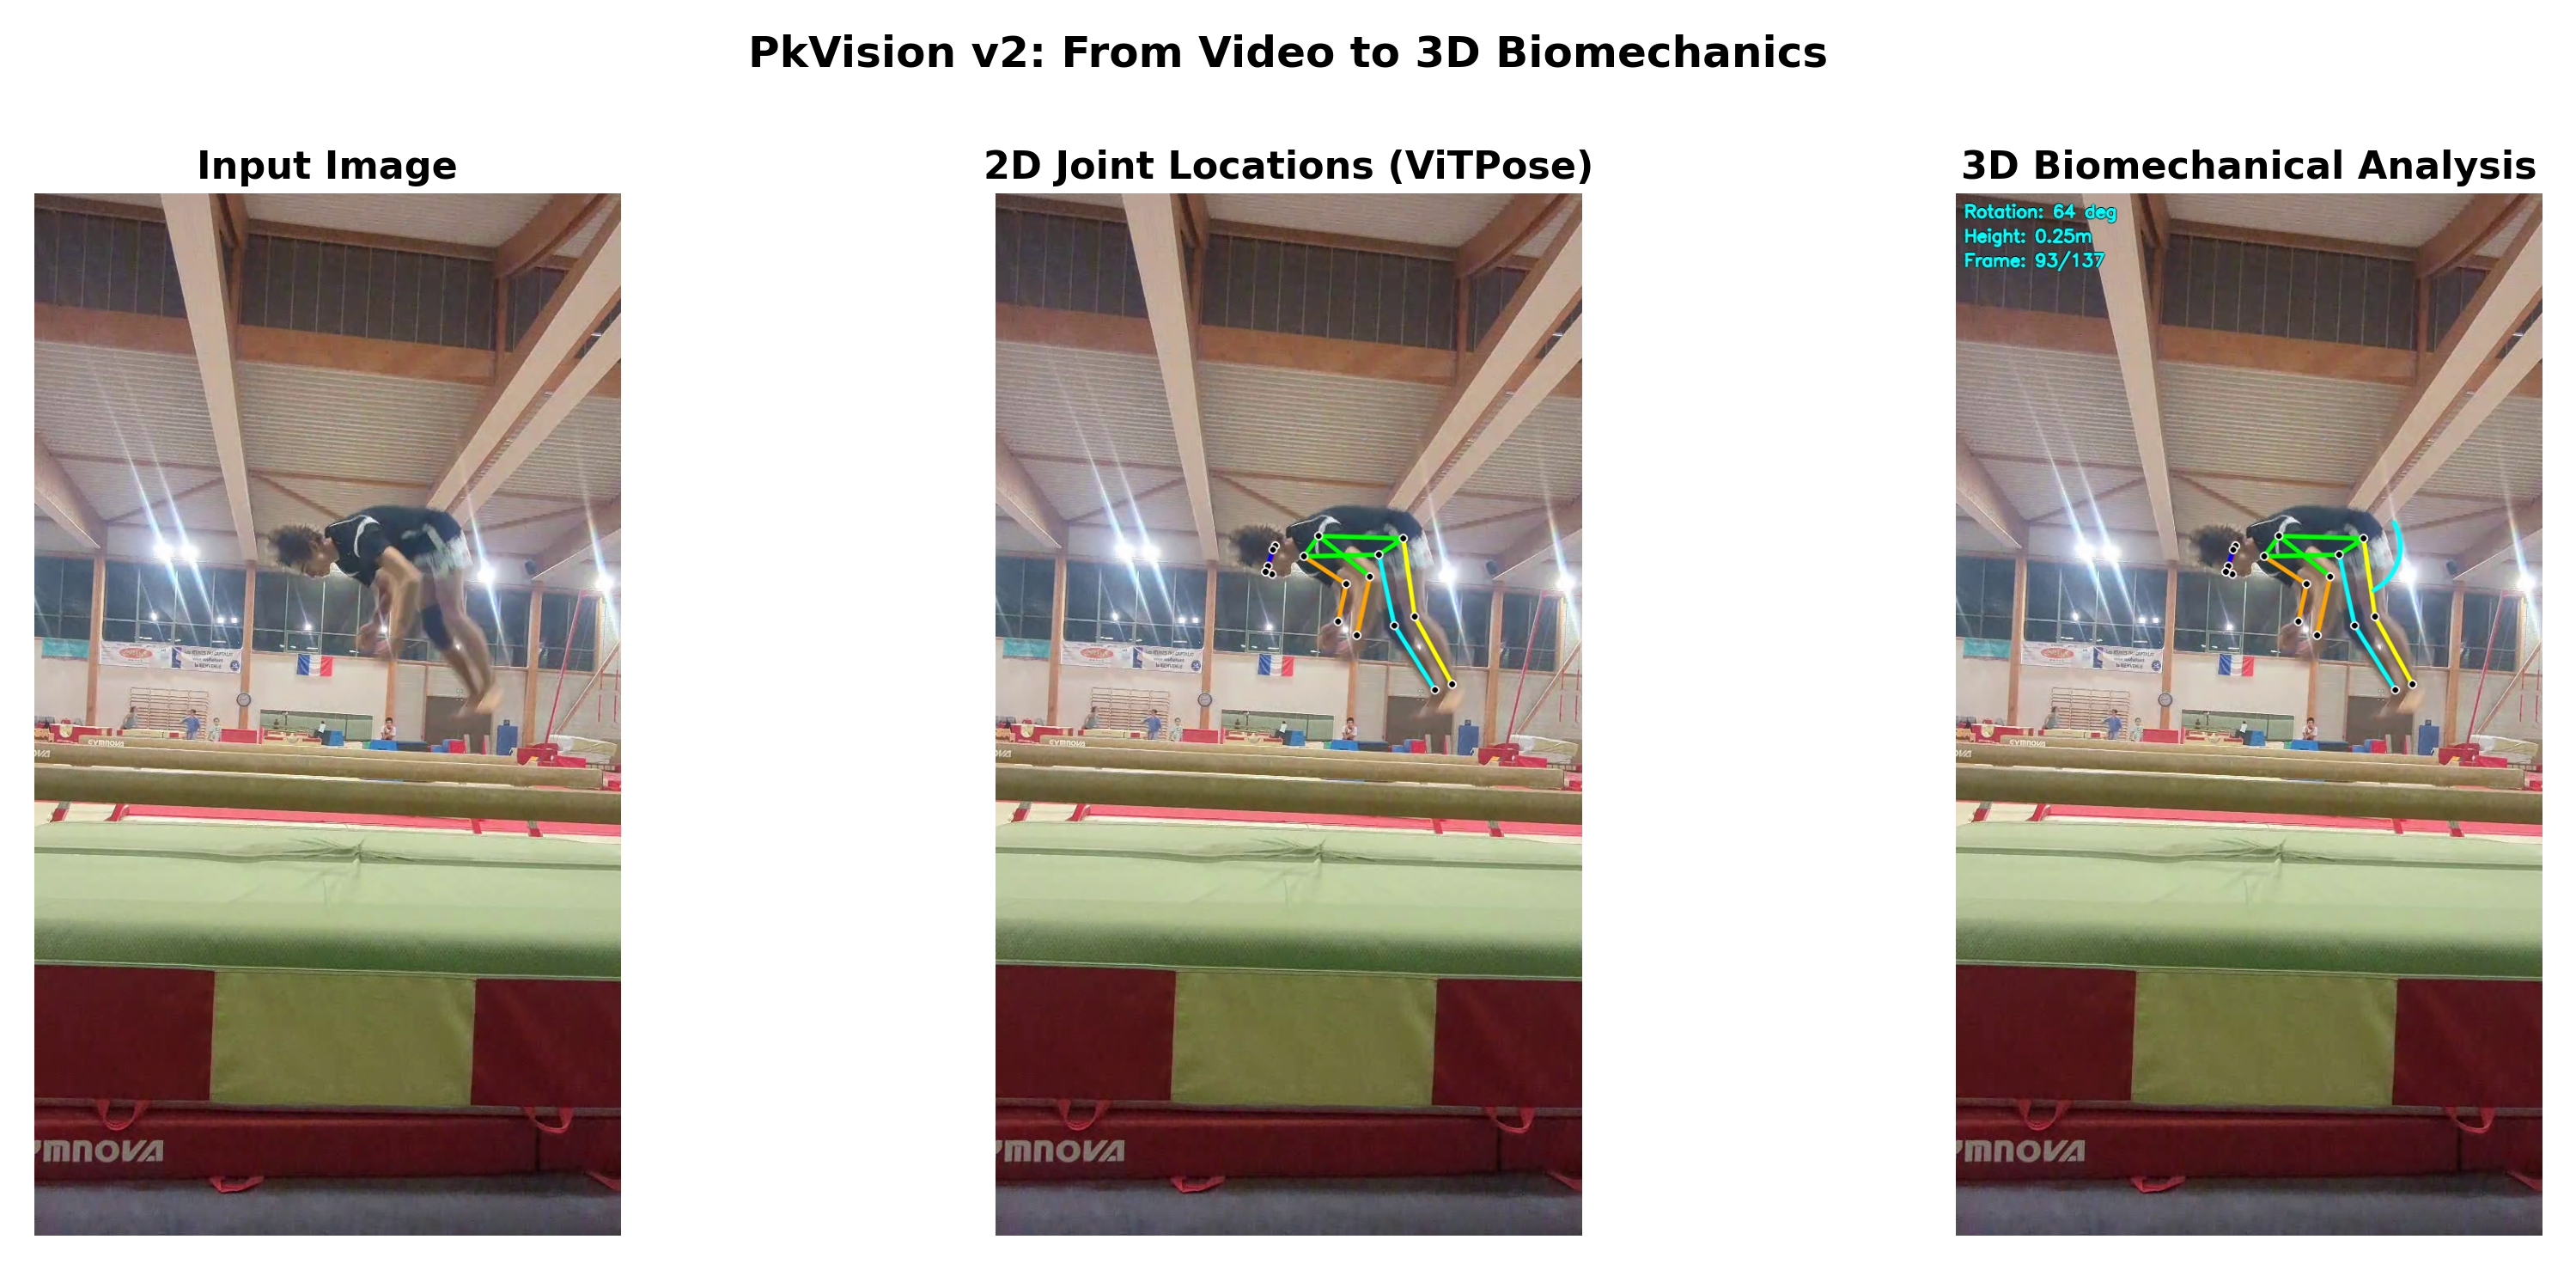
\includegraphics[width=\linewidth]{figures/fig06_gvhmr_failure.png}
  \caption{\textbf{GVHMR on acrobatic footage.} Left: clean back flip,
  mesh well-aligned, flip count $= 0.98$. Middle: gainer full, twist axis
  drifts as the body passes through inversion. Right: double cork, total
  rotation reports 3.97 revolutions against a ground truth of 2.5, and body
  orientation is unrecoverable. The model inherits AMASS's distributional
  gap; no amount of post-processing recovers the signal.}
  \label{fig:gvhmr_failure}
\end{figure}

\paragraph{v5a --- Metric learning on parkourtheory clips.}
We scraped \num{1618} labeled single-trick clips from
parkourtheory.com, grouped them into 43 trick families, and fine-tuned
VideoMAE~\cite{tong2022videomae} with a batch-hard triplet loss and a
$P{=}4, K{=}2$ sampler. After 50 epochs of training on Modal T4 instances,
Recall@1 plateaued at 9\%; on closer inspection the embedding space had
collapsed and every query resolved to the same family. The dataset is
simply too small and too diverse for metric learning to find stable
margins. A quantitative summary of both this and the attribute classifier approach is
given directly in the text above.

\paragraph{v5b --- Hierarchical attribute classifiers.}
Instead of full trick identification, we trained four heads on the
VideoMAE backbone to predict attributes: context (acrobatics / wall /
swing / pk\_basics), direction, flip bin, and twist bin. Mean per-attribute
accuracy reached 55\% after six epochs before a scheduled cluster time-out
terminated the run. The trend was still improving, but at the measured rate
per-epoch $(\approx\!31$\,min on an RTX 2060$)$ the compute budget did not
justify continuing: even a strong attribute classifier would not reach the
level of a FIG judge, and adding new tricks would still require retraining.

\paragraph{CLIP zero-shot baseline.}
As a baseline we also evaluated CLIP ViT-B/32~\cite{radford2021clip} in a
zero-shot configuration, scoring each clip against text prompts of the form
\emph{``a video of a \texttt{<trick>} being performed''}. Accuracy on
four-way categorical attributes landed between 37\% and 48\%; exact-trick
top-1 on a 10-clip held-out slice was 0\%. CLIP has sufficient vocabulary
for coarse categories but no representation of the compositional
trick-naming system that the parkour community actually uses.

\paragraph{What all failures had in common.}
Every trained approach fell into the same trap. The 1\,600-clip training
set is vast for a hobby and tiny for a deep model. The label space (1\,837
distinct trick names, 193 unique physics combinations) has extreme class
imbalance. Most critically, FIG trick names are \emph{linguistic}: they
encode a shared taxonomy among athletes and judges, not a purely kinematic
one. A VLM trained on billions of web pages has already absorbed that
taxonomy for free. That observation, together with Claude and Gemini's
correct identification of the tricks in \texttt{IMG\_5985.mov} on the first
attempt, is what motivated the pivot described in Sec.~\ref{sec:system}.
